\documentclass[pdftex,12pt,a4paper]{article}
\usepackage[utf8]{inputenc}
\usepackage[T1]{fontenc}
\usepackage{lmodern}
\usepackage{tabularx}
\usepackage{graphicx}
\usepackage{hyperref}
\usepackage[ngerman]{babel}
\usepackage{booktabs,paralist}
\usepackage{scrpage2,lastpage}


\begin{document}

%Titelblatt
\begin{titlepage}
\begin{center}
\textsc{\LARGE Technische Universit\"at Dresden} \\[0.5cm]
\textsc{\LARGE Softwaretechnologie-Projekt\\[0.2cm]Gruppe 30}\\[0.7cm]
\textsc{\LARGE Geek-Shop}\\[4cm]
{\fontsize{35}{35} \bfseries Benutzerhandbuch}\\
\vspace*{\fill}
Sebastian D\"oring, Felix D\"oring, Marcus Kammerdiener,\\ Dominik Lauck, Elizaveta Ragozina\\[0.5cm]
\url{http://is63050.inf.tu-dresden.de/~swt14w30/index.php}
\end{center}
\end{titlepage}


%Inhaltsverzeichnis
\tableofcontents
\newpage

%Zielbestimmung
\section{Zielbestimmung}
Durch Einsatz des Produktes sollen Mitarbeiter des Geek-Shops "`Think Nerd"' den Kassenbetrieb elektronisch an B\"urorechnern verwalten.
\subsection*{Muss-Kriterien}
\begin{itemize}
\item An- und Abmeldesystem
\item Passwortverwaltung
\item Passwortverschl\"usselung
\item Bemnutzerverwaltung
\item Witzverwaltung
\item Artikel- und Artikelkategorienverwaltung
\item Warenkorbverwaltung
\item Verkaufsabwicklung
\item Ausw\"ahlen der Zahlungsmethode
\item Rechnungserstellung
\item Lagerbestandsverwaltung
\item Setzen der unteren Grenze des Bestandes f\"ur Artikel durch den Ladenbesitzer
\item Warung bei Unterschreitung der unteren Grenze
\item XML-Exportfunktion f\"ur Verkaufsdaten
\end{itemize}
\subsection*{Kann-Kriterien}
\begin{itemize}
\item Automatische Abmeldung nach einer bestimmten Zeit
\item Vermeidung sich wiederholender Witze
\end{itemize}
\subsection*{Abgrenzungskriterien}
\begin{itemize}
\item Maximal zweisprachiges Webinterface
\item Bedienung nur durch Mitarbeiter des Shops
\end{itemize}

%Produkteinsatz
\section{Produkteinsatz}
Das Produkt wird auf B\"urorechnern des Ladenbesitzers und der Kasse installiert. Die Angestellten k\"onnen dadurch die Kaufabwicklung betreiben. Dem Ladenbesitzer stehen zus\"atzlich die Administratorenfunktionen zur Verf\"ugung. Er kann Sortiment-, Angestellten- und Lagerbestandsverwaltung betreiben. Hier sei auf das Anwendungsfalldiagramm verwiesen.
\subsection*{Zielgruppen}
\begin{itemize}
\item Angestellte: Verkaufs- und Reklamationsabwicklung
\item Ladenbesitzer: Funktionen des Angestellten und Sortiment-, Angestellten- und Lagerbestandsverwaltung.
\end{itemize}
\subsection*{Betriebsbedingungen}
Das Produkt wird auf den B\"urorechnern an der Kasse des Shops betrieben. Alle Mitarbeiter haben durch einen eigenen Account Zugriff auf das System.

%Produktuebersicht
\section{Produkt\"ubersicht}
\subsection*{Anwendungsfalldiagramm}
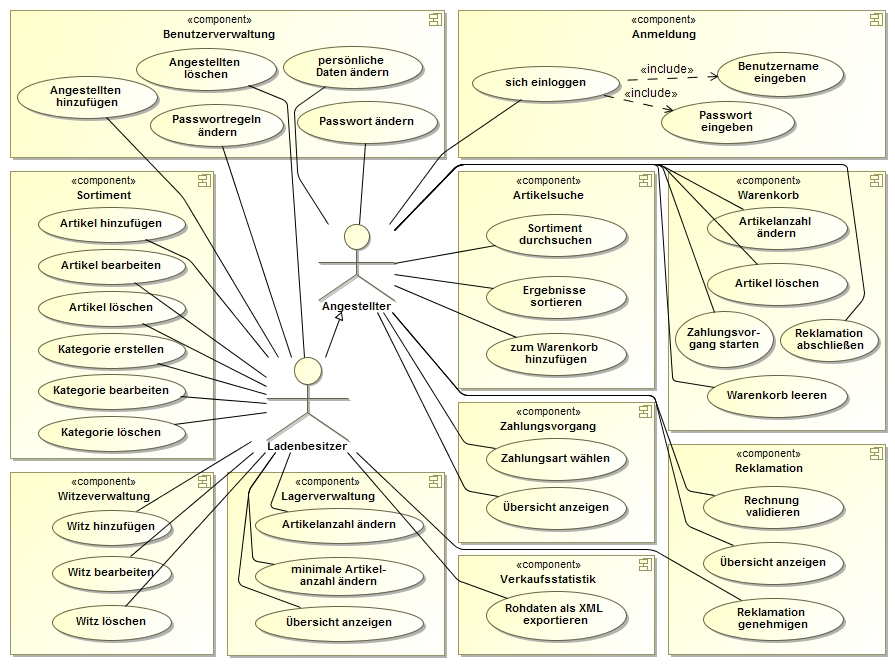
\includegraphics[width=1\textwidth]{./images/anwendungsfalldiagramm}
Das Anwendungsfalldiagramm zeigt die in die verschiedenen Teilbereiche gegliederten Anwendungsf\"alle, mit denen sich die Akteure des Systems konfrontiert sehen.
\subsection*{Sequenzdiagramme}
\subsubsection*{1. Anmeldung}
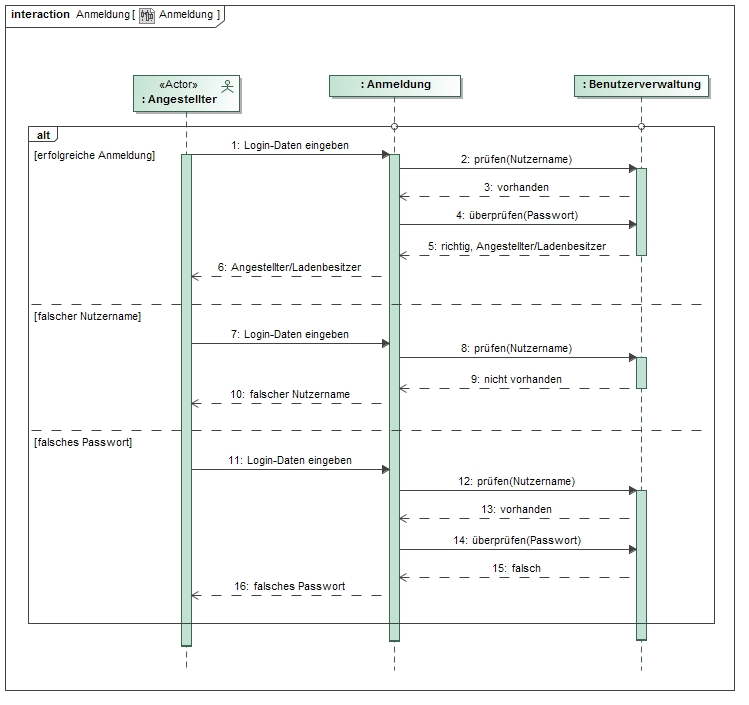
\includegraphics[width=1\textwidth]{./images/anmeldung}
Dieses Diagramm beschreibt den Anmeldevorgang des Benutzers und wie das Programm bei einem fehlerhaften Benutzernamen oder Passwort reagiert.
\subsubsection*{2. Witze}
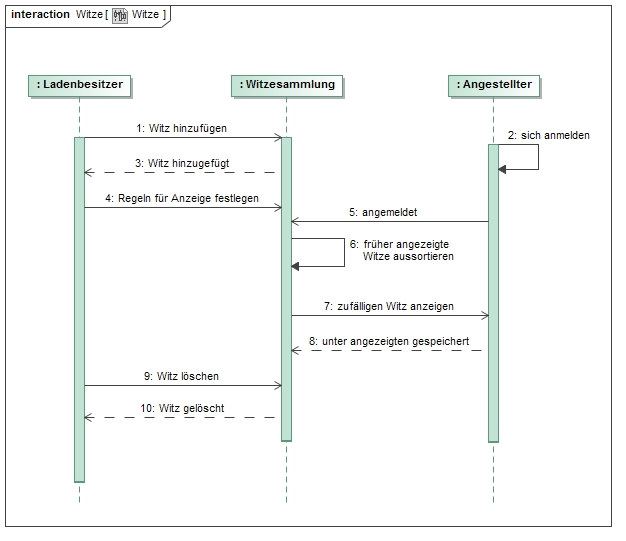
\includegraphics[width=1\textwidth]{./images/witze}
Im folgenden Diagramm wird gezeigt, wie der Ladenbesitzer einen neuen Witz zur bestehenden Witzsammlung hinzufügen kann, wie ein zufälliger Witz aus der Sammlung einem Angestellten angezeigt wird und wie ein Witz aus der Sammlung gelöscht wird.
\subsubsection*{3. Benutzerverwaltung}
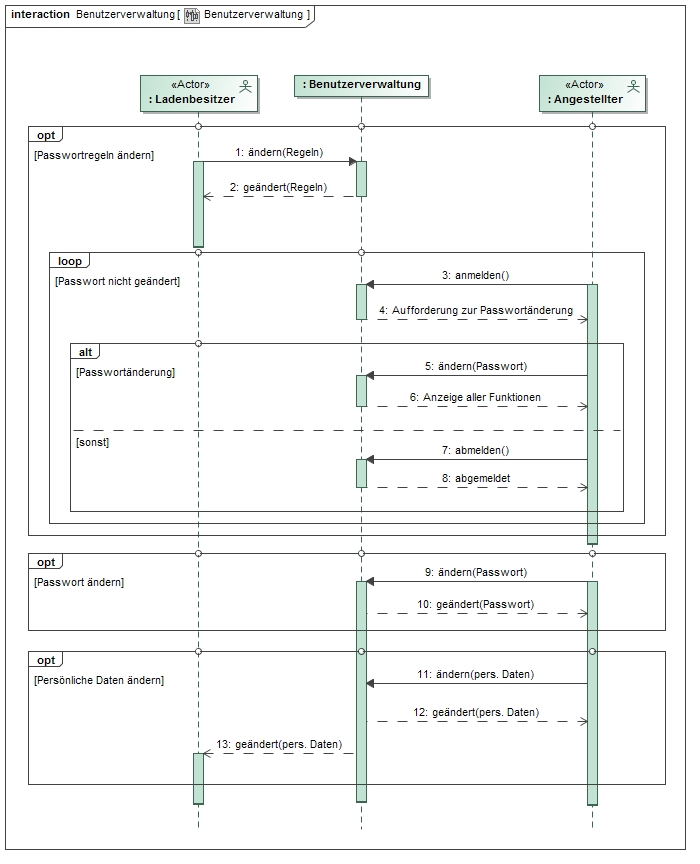
\includegraphics[width=1\textwidth]{./images/benutzerverwaltung}
In dem Sequenzdiagramm der Benutzerverwaltung werden die M\"oglichkeit der \"Anderung der pers\"onlichen Daten und das Setzen neuer Passwortregeln sowie die dazugeh\"orige \"Anderung des Passwortes beschrieben.
\subsubsection*{3.1 Angestellten hinzuf\"ugen}
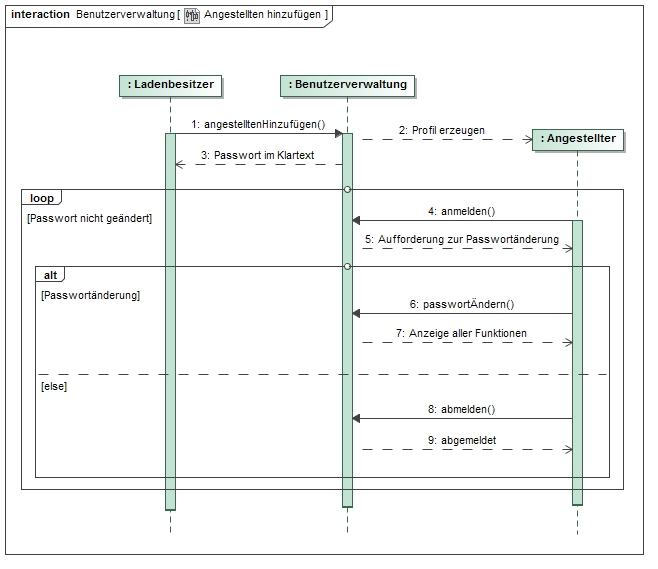
\includegraphics[width=1\textwidth]{./images/angestelltenhinzufuegen}
Das Sequenzdiagramm zeigt den Ablauf und die Interaktion zwischen den Objekten des Systems f\"ur den Fall, dass ein neuer Mitarbeiter angelegt wird.
\subsubsection*{3.2 Angestellten l\"oschen}
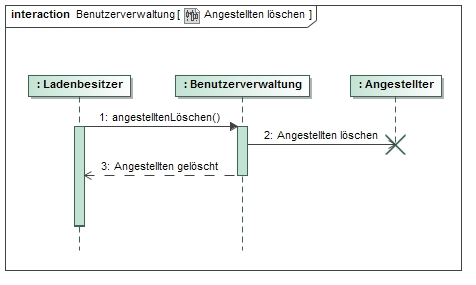
\includegraphics[width=1\textwidth]{./images/angestelltenloeschen}
Das Sequenzdiagramm zeigt den Ablauf und die Interaktion zwischen den Objekten des Systems f\"ur den Fall, dass ein neuer Mitarbeiter gel\"oscht wird.
\subsubsection*{4. Kaufvorgang}
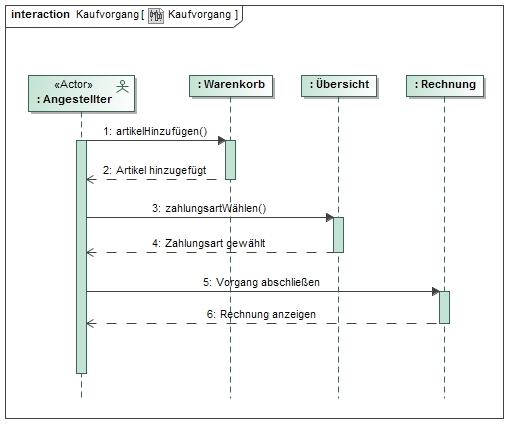
\includegraphics[width=1\textwidth]{./images/kaufvorgang}
Dieses Diagramm zeigt, wie ein \"ublicher Kaufvorgang abl\"auft.
\subsubsection*{5. Reklamation}
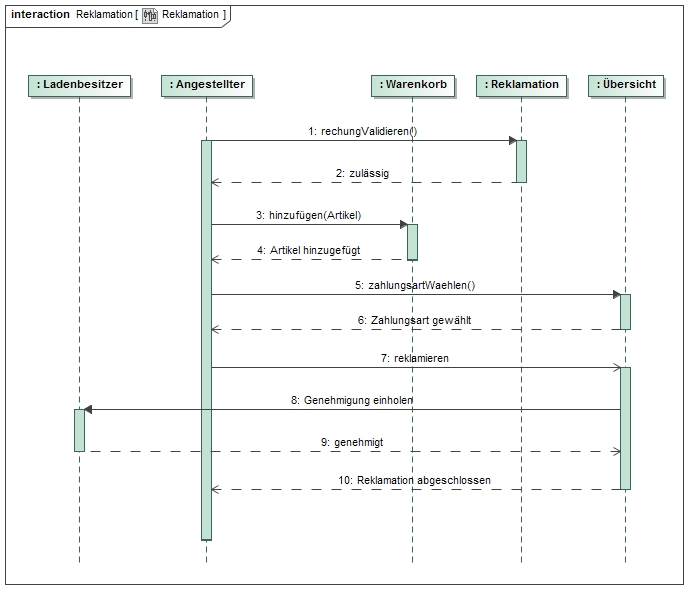
\includegraphics[width=1\textwidth]{./images/reklamation}
Hier wird beschrieben, wie eine Reklamation abl\"auft.
\subsection*{Top-Level-Architektur}
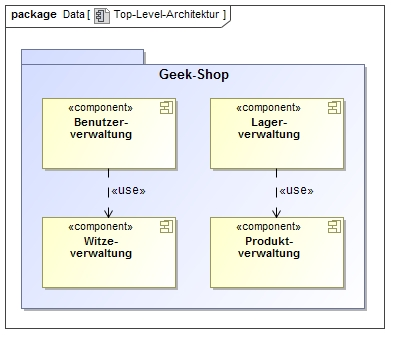
\includegraphics[width=1\textwidth]{./images/toplevelarchitektur}
Die Top-Level-Architektur veranschaulicht die inneren Komponenten des Shops und ihre Abh\"angigkeiten untereinander auf oberster Ebene.
\subsection*{Analyseklassendiagramm}
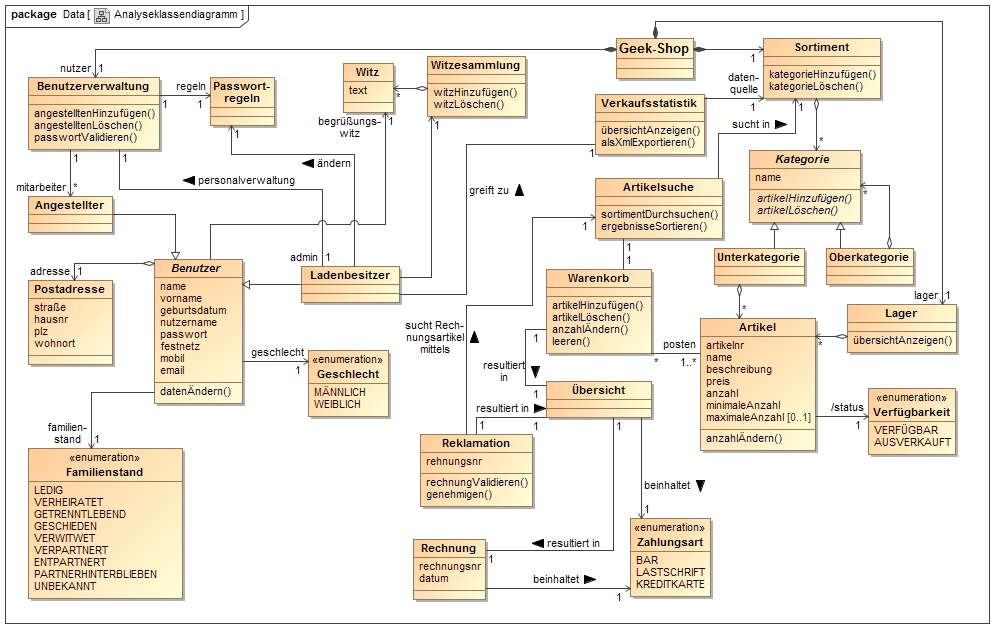
\includegraphics[width=1\textwidth]{./images/analyseklassendiagramm}
Das Analyseklassendiagramm zeigt die Klassen und Beziehungen des Systems, die sich aus dem Kundengespr\"ach ergeben haben. \\
Klassenbeschreibung: \\
\begin{itemize}
\item Die Klasse Geek-Shop vereint die groben Bestandteile des Shops. Sie besteht aus Benutzerverwaltung, Sortiment und Lager.
\item Die Klasse Ladenbesitzer bildet den realen Ladenbesitzer ab. Sie ist für die Verwaltung des Shops verantwortlich. Insbesondere kümmert er sich um Personalverwaltung, Witzeverwaltung, Passwortregeln und Verkaufsstatistik. Die Klasse erbt von Benutzer.
\item Die Klasse Benutzerverwaltung verwaltet die Angestellten und den Ladenbesitzer. Weiterhin umfasst sie Funktionalit\"aten der Personalverwaltung.
\item Die Klasse Angestellter abstrahiert die Mitarbeiter des Shops. Allgemeine Eigenschaften werden von der Klasse Benutzer geerbt.
\item In der abstrakten Klasse Benutzer sind die typischen Eigenschaften eines Angestellten und des Ladenbesitzers zusammengefasst. Die Postadresse ist als separate Klasse modelliert. Enumerationen f\"ur Geschlecht und Familienstand sind weitere Benutzereigenschaften. Jedem Benutzer ist ein Passwort zugewiesen, das mithilfe der Passwortregeln auf ausreichende Sicherheit gepr\"uft wird.
\item Die Klasse Witz, deren Objekte von der Klasse Witzesammlung verwaltet werden, stellt die Witze dar, die die Angestellten nach dem Login angezeigt bekommen.
\item Die Klasse Sortiment umfasst die verschiedenen Produktkategorien mit den darin enthaltenen Artikeln.
\item Die abstrakte Klasse Kategorie abstrahiert die Kategorien, deren Eigenschaften und Funktionalitäten.
\item Die Klassen Oberkategorie und Unterkategorie erben von Kategorie. Oberkategorie stellt eine Kategorie dar, die weitere Kategorien als Unterkategorien enthält. Unterkategorie hingegen enthält ausschließlich Artikel.
\item Die Klasse Artikel bildet Waren ab. Das abgeleitete Attribut status als Wert der Enumeration Verfügbarkeit gibt die Verfügbarkeit des Artikels an.
\item Die Klasse Lager repräsentiert das Lager des Shops, wo die Artikel gelagert sind.
\item Die Klasse Warenkorb stellt den Warenkorb dar, der mit Artikeln gefüllt wird. Die Klasse enthält dafür benötigte Operationen.
\item Die Artikel des Warenkorbs werden mithilfe der Artikelsuche (repräsentiert durch die gleichnamige Klasse) im Sortiment gefunden.
\item Die Klasse Übersicht abstrahiert die Übersicht, die alle wichtigen Informationen des Kundenauftrages anzeigt.
\item Die Klasse Rechnung repräsentiert die Rechnung, die abschließend angezeigt wird.
\item Die Klasse Reklamation stellt grundlegende Funktionalitäten für die Reklamation von Artikeln bereit.
\item Mithilfe der Klasse Verkaufsstatistik kann vom Ladenbesitzer abgerufen werden, welcher Artikel wann in welcher Menge verkauft wurde.
\end{itemize}
\subsection*{Dialoglandkarte}
\includegraphics[width=1\textwidth]{./images/dialoglandkarte}
\newpage

%Produktfunktionen
\section{Produktfunktionen}
\subsubsection*{/F01/ Begr\"u\ss{}ung}
\begin{itemize}
\item Nach Anmeldung eines Angestellten zeigt das System eien zuf\"alligen Nerdwitz. Dabei werden die f\"unf zuletzt gezeigten Witze aus der Auswahl ausgeschlossen.
\item Der Ladenbesitzer kann Witze hinzuf\"ugen
\item Der Ladenbesitzer kann Witze bearbeiten
\item Der Ladenbesitzer kann Witze l\"oschen
\end{itemize}
\subsection*{Account}
\subsubsection*{/F02/ Profilverwaltung}
\begin{itemize}
\item Der Ladenbesitzer kann neue Profile erstellen
\item Der Ladenbesitzer kann Profile l\"oschen (entlassen)
\item Der Ladenbesitzer kann Profilinformationen bearbeiten
\end{itemize}
\subsubsection*{/F03/ Passwortverwaltung}
\begin{itemize}
\item Der Ladenbesitzer kann Passwortregeln beim Aufsetzen des Systems festlegen (min/max Zeichenanzahl, Gro\ss{}buchstaben ja/nein, Sonderzeichen ja/nein)
\item Der Ladenbesitzer kann Passwortregeln \"andern. Die Angestellten werden bei der Anmeldung aufgefordert, ihr Passwort nach den neuen Regeln zu \"andern
\item Alle Mitarbeiter k\"onnen jederzeit ihr Passwort nach den g\"ultigen Regeln \"andern
\item Der Ladenbesitzer wird \"uber Passwort\"anderungen anderer Angestellter benachrichtigt
\item Der Ladenbesitzer kann jederzeit Passw\"orter anderer Angestellter \"andern
\item Alle Passw\"orter sind verschl\"usselt
\end{itemize}
\subsection*{Sortiment}
\subsubsection*{/F020/ Verwaltung von Artikeln}
\begin{itemize}
\item Mitarbeiter k\"onnen nach Artikeln suchen
\item Mitarbeiter k\"onnen Artikel nach Name und Preis sortieren (auf-/absteigend)
\item Mitarbeiter k\"onnen Informationen zu jedem Artikel lesen
\item Der Ladenbesitzer kann neue Artikel erstellen
\item Der Ladenbesitzer kann Artikel bearbeiten
\item Der Ladenbesitzer kann Artikel l\"oschen
\item Der Ladenbesitzer kann Kategorien und Unterkategorien erstellen
\item Der Ladenbesitzer kann Kategorien und Unterkategorien umbenennen
\item Der Ladenbesitzer kann Kategorien und Unterkategorien l\"oschen
\end{itemize}
\subsubsection*{/F050/ Lagerbestandsverwaltung}
\begin{itemize}
\item Der Ladenbesitzer kann Mengen von Artikeln \"andern
\item Der Ladenbesitzer kann nach Artikeln suchen
\item Der Ladenbesitzer kann eine untere Grenze f\"ur Bestand der Artikel setzen
\item Der Ladenbesitzer wird bei unterschreitung der unteren Grenze gewarnt
\item Der Ladenbesitzer kann Verkaufsdaten einsehen und mit Hilfe der XML-Exportfunktion exportieren
\end{itemize}
\subsection*{Kaufabwicklung}
\subsubsection*{/F060/ Warenkorbverwaltung}
\begin{itemize}
\item Mitarbeiter k\"onnen jeden Artikel in den Warenkorb legen
\item Mitarbeiter k\"onnen jeden Artikel aus dem Warenkorb entfernen
\item Mitarbeiter k\"onnen den Warenkorb leeren
\item Mitarbeiter k\"onnen hineingelegte Artikel ansehen
\item Mitarbeiter k\"onnen die Anzahl von Artikeln \"andern
\item Zahlungsvorgang starten
\item Reklamation abschlie\ss{}en
\end{itemize}
\subsubsection*{/F070/ Bezahlvorgang}
\begin{itemize}
\item Zahlungsmethode ausw\"ahlen (Kreditkarte, Bar, Lastschrift)
\item Kundendaten eingeben
\item Verkaud best\"atigen
\item Rechnung anzeigen
\end{itemize}
\subsubsection*{/F080/ Reklamation}
\begin{itemize}
\item Rechnung validieren
\item \"Ubersicht anzeigen
\item Der Ladenbesitzer kann Reklamationen genehmigen und somit abschlie\ss{}en
\item Der Ladenbesitzer kann Reklamationen ablehnen
\end{itemize}

%Produktdaten
\section{Produktdaten}
Folgende Daten sind \"uber einzelne Elemente zu speichern:
\subsubsection*{/D010/ Profil}
\begin{itemize}
\item Name
\item Adresse
\item Geburtsdatum
\item Telefonnummer
\item Email-Adresse
\item Geschlecht
\item Familienstand
\item Benutzername
\item Passwort
\end{itemize}
\subsubsection*{/D020/ Artikel}
\begin{itemize}
\item Name
\item Preis
\item Kategorie
\item (gegebenenfalls) Unterkategorie
\item Artikelnummer
\item Verf\"ugbarkeit
\end{itemize}
\subsubsection*{/D030/ Lagereintrag}
\begin{itemize}
\item Eintrags-ID
\item Vorhandene Anzahl
\item Untere Grenze
\end{itemize}
\subsubsection*{/D040/ Witz}
\begin{itemize}
\item Witz-Inhalt
\item Witz-ID
\end{itemize}
\subsubsection*{/D050/ Warenkorb}
\begin{itemize}
\item ID von reingelegten Artikeln
\item Anzahl von jedem Artikel
\end{itemize}
\subsubsection*{/D060/ Verkaufsvorgang}
\begin{itemize}
\item K\"auferdatem
\item ID der gekauften Artikel
\item Datum
\item Bezahlmethode
\end{itemize}

%Qualitaetsanforderungen
\section{Qualit\"atsanforderungen}
\begin{tabularx}{\textwidth}{| *4{>{\centering\arraybackslash}X|}} \hline
{\textbf{Produktivit\"at}} & {\textbf {sehr gut}} & {\textbf {gut}} & {\textbf {normal}}\\ \hline
Funktionalit\"at & & X & \\ \hline
Zuverl\"assigkeit & X & & \\ \hline
Effizienz & & & X \\ \hline
Behutsamkeit & X & & \\ \hline
\"Anderbarkeit & & X & \\ \hline
\end{tabularx}
\end{document}